\documentclass[conference]{IEEEtran}
\usepackage[utf8]{inputenc}
\usepackage[T1]{fontenc}
\usepackage{amsmath,amssymb}
\usepackage{graphicx}
\usepackage{hyperref}
\usepackage{booktabs}
\usepackage{titlesec}
\usepackage[spanish]{babel}
\usepackage{tikz}
\usetikzlibrary{arrows.meta,positioning,shapes.geometric,babel}

% Formato de secciones: numeración arábiga, alineación izquierda y negrita.
\titleformat{\section}[hang]
  {\normalfont\large\bfseries\raggedright}
  {\arabic{section}.}
  {0.6em}
  {}

\titleformat{\subsection}[hang]
  {\normalfont\fontsize{11}{13}\selectfont\bfseries\raggedright}
  {\arabic{section}.\arabic{subsection}}
  {0.6em}
  {}

\hypersetup{
  colorlinks=true,
  linkcolor=black,
  citecolor=black,
  urlcolor=black
}


\title{Position Paper: AutoML Multiagéntico para la Generación de Pipelines Auditables y Explicables}

\author{
\IEEEauthorblockN{Jonnathan Cuzco, Joshua Cueva, Juan Coronel, Víctor Saquicela}
\IEEEauthorblockA{Universidad de Cuenca\\
\{jonathan.cuzcot, joshua.cueva, juan.coronelc, victor.saquicela\}@ucuenca.edu.ec}
}

\begin{document}

\maketitle

\begin{abstract}
Las herramientas actuales de automatización del aprendizaje automático (AutoML) aceleran la selección de algoritmos y la optimización de hiperparámetros, pero operan fundamentalmente como cajas negras: no razonan semánticamente sobre los datos, no justifican sus decisiones algorítmicas y carecen de la trazabilidad exigida por entornos altamente regulados. Este artículo de posición propone un sistema AutoML multiagéntico que integra agentes MCP especializados basados en LLMs, ontologías formales, y aprendizaje por refuerzo jerárquico para generar pipelines de ML con explicabilidad. La propuesta opera mediante dos fases complementarias: un entorno de simulación estocástica donde los agentes exploran iterativamente, y acumulan conocimiento empírico para entrenar políticas de aprendizaje por refuerzo; y una fase de producción determinista que ejecuta la estrategia aprendida con total transparencia. Crucialmente, la arquitectura incorpora agentes XAI y un agente generador de reportes que integra cada decisión y hallazgo en un reporte interpretable. Esta propuesta redefine el estado del arte, sentando las bases para una IA autónoma que no solo optimiza métricas de rendimiento, sino que justifica sus decisiones y audita sus propias acciones.
\end{abstract}

\begin{IEEEkeywords}
AutoML, Sistemas Multiagente, Ontologías, Aprendizaje por Refuerzo, XAI, LLM, GraphRAG.
\end{IEEEkeywords}

\section{Introducción}

En el mundo digital contemporáneo, los datos constituyen el activo subyacente de mayor valor estratégico. El Machine Learning (ML) se ha posicionado como una tecnología fundamental para extraer conocimiento accionable de estos repositorios masivos de datos \cite{he2021automl}, impulsando decisiones en diagnósticos médicos, modelos de riesgo financiero, predicciones del clima y un sinfín de dominios donde la identificación de patrones latentes define el éxito competitivo~\cite{baratchi2024}.

Sin embargo, la construcción de modelos de ML de grado industrial sigue siendo un proceso altamente artesanal. Requiere seleccionar algoritmos idóneos entre cientos de candidatos, diseñar características complejas, ajustar hiperparámetros de forma minuciosa y validar cada decisión arquitectónica \cite{doke2021automl}. Este ciclo de desarrollo iterativo consume enormes recursos computacionales y temporales de ingenieros altamente especializados, está sujeto a sesgos heurísticos humanos y, lo que es más crítico para la industria, raramente genera una bitácora auditable que justifique por qué se eligió una metodología~\cite{wu2022survey}.

La automatización del ML (AutoML) surgió con la promesa de eliminar este cuello de botella~\cite{hutter2019}. Plataformas consolidadas como Auto-Sklearn~\cite{feurer2019}, AutoGluon~\cite{erickson2020} y Auto-WEKA~\cite{kotthoff2017} han logrado sistematizar la búsqueda de pipelines mediante optimización bayesiana y meta-aprendizaje, liberando a los científicos de datos de la exploración manual. No obstante, tras más de una década de maduración tecnológica, el paradigma del AutoML clásico exhibe tres limitaciones estructurales severas que impiden su adopción masiva en ecosistemas empresariales de misión crítica.

Primero, estas herramientas tratan los conjuntos de datos como matrices numéricas, ignorando la semántica del dominio. Aunque un problema de abandono de clientes y uno de falla estructural de turbinas puedan parecer similares matemáticamente, requieren tratamientos distintos desde el punto de vista semántico~\cite{barbudo2023}. Segundo, el AutoML tradicional funciona como una caja negra; el usuario recibe un modelo optimizado y una métrica de precisión, pero no conoce las transformaciones aplicadas ni las relaciones que el sistema utilizó~\cite{gundersen2018}. Tercero, muchas herramientas generan arquitecturas rígidas y poco transparentes \cite{zou2025metalearning}, incompatibles con los requisitos de Inteligencia Artificial Explicable (XAI) y con las exigencias de gobernanza algorítmica en sectores como el corporativo, financiero y de la salud.

De manera simultánea, la inteligencia artificial está experimentando una transición paradigmática impulsada por los Modelos de Lenguaje de Gran Escala (LLMs). Estos modelos han evolucionado de simples motores probabilísticos de texto a agentes autónomos dotados de capacidades de planificación, uso de herramientas y razonamiento complejo~\cite{wang2025llmagent,yao2023react}. Ecosistemas vanguardistas como AutoGen~\cite{wu2023autogen} demuestran que la orquestación de múltiples agentes especializados, interactuando bajo protocolos semánticos estrictos, permite resolver problemas intrincados minimizando las alucinaciones inherentes a los modelos monolíticos~\cite{huang2023mlagentbench}.

Este artículo de posición propone una arquitectura multiagente para evolucionar la automatización del aprendizaje automático. En lugar de limitarse a una optimización ciega, el sistema propuesto razona lógicamente sobre los datos mediante un motor ontológico, experimenta autónomamente en un entorno seguro y aprende de sus interacciones mediante aprendizaje por refuerzo jerárquico (HRL). En su fase de producción, genera pipelines deterministas con trazabilidad total y redacta informes narrativos que explican las decisiones tomadas y las variables clave del modelo. El resultado es un sistema preparado para el escrutinio empresarial, capaz de transicionar el AutoML desde la simple eficiencia algorítmica hacia la confianza, la explicabilidad y la autonomía auditable, facilitando la interpretabilidad de modelos de aprendizaje automático.

\section{Escenario}
En una empresa de distribución o comercio electrónico, decisiones como cuánto inventario mantener, qué precio asignar a un producto o cuándo ajustar el margen de una categoría se toman constantemente y pueden afectar directamente las ventas y la rentabilidad. Para apoyar estas decisiones, el AutoML permite automatizar la construcción de modelos predictivos y encontrar configuraciones que ofrecen un buen desempeño. Sin embargo, para un usuario del negocio, obtener una buena predicción no siempre es suficiente: también necesita entender por qué el sistema recomienda una determinada acción, qué factores influyeron en el resultado y si la recomendación es coherente con la realidad del negocio. Cuando estas soluciones no incorporan el conocimiento que los usuarios tienen sobre su dominio ni ofrecen explicaciones claras, resulta más difícil confiar en sus resultados y utilizarlos para tomar decisiones. Por ello, el desafío consiste en avanzar hacia sistemas de AutoML que no solo busquen modelos precisos, sino que también incorporen conocimiento del dominio y proporcionen explicaciones comprensibles y trazables. Aunque este problema se plantea en el contexto comercial, el mismo enfoque puede aplicarse a otros dominios donde las decisiones automatizadas requieren conocimiento especializado, confianza y capacidad de explicar cómo se llegó a una recomendación.

Para fundamentar científicamente la solución a este desafío, es necesario analizar la trayectoria tecnológica del AutoML y precisar la brecha estructural que impide a los sistemas actuales alcanzar esta visión.

Las primeras generaciones de AutoML buscaron resolver la Selección Combinada de Algoritmos y Optimización de Hiperparámetros (CASH) mediante optimización bayesiana y búsqueda heurística~\cite{thornton2013}. Herramientas como Auto-WEKA~\cite{kotthoff2017} demostraron que la búsqueda automatizada podía superar estrategias manuales en escenarios controlados. A partir de ahí, Auto-Sklearn incorporó meta-aprendizaje para aprovechar el conocimiento de conjuntos de datos similares~\cite{feurer2019}, mientras que AutoGluon amplió el enfoque con ensamblajes multicapa orientados a maximizar la exactitud predictiva~\cite{erickson2020} y Auto-Keras lo llevó al ámbito de la búsqueda automática de arquitecturas neuronales~\cite{jin2019}. En conjunto, estos avances demostraron que la automatización podía igualar e incluso superar el diseño humano de pipelines en determinados escenarios.


Sin embargo, la literatura reciente evidencia limitaciones estructurales en estos enfoques~\cite{barbudo2023,baratchi2024}. Aunque son optimizadores altamente eficientes, operan principalmente como procesos de búsqueda secuenciales con una comprensión limitada del contexto del problema. No incorporan razonamiento semántico sobre el dominio, presentan dificultades para adaptarse a restricciones externas y carecen de mecanismos robustos para justificar sus decisiones ante usuarios expertos o procesos de auditoría~\cite{gundersen2018}. En esencia, optimizan configuraciones, pero no comprenden por qué una solución resulta adecuada.

La integración de Modelos de Lenguaje Grandes (LLMs) introdujo una nueva etapa al permitir interpretar instrucciones en lenguaje natural y generar código de ML de manera iterativa~\cite{wang2025llmagent}. Paradigmas como ReAct~\cite{yao2023react} incorporaron capacidades de razonamiento, planificación y uso de herramientas externas, mientras que sistemas como PandasAI demostraron su utilidad para asistir procesos analíticos dinámicos. No obstante, delegar la construcción completa de un pipeline a un único agente LLM presenta problemas de escalabilidad, consistencia y confiabilidad debido a la saturación del contexto, las alucinaciones y la falta de determinismo~\cite{huang2023mlagentbench,hong2024datainterpreter}.

Como respuesta a estas limitaciones surgieron los Sistemas Multiagente (MAS), donde la complejidad se distribuye entre agentes especializados con responsabilidades diferenciadas~\cite{balaji2010}. Frameworks como AutoGen~\cite{wu2023autogen} y MetaGPT~\cite{hong2023metagpt} demostraron que la colaboración entre agentes permite incorporar mecanismos de revisión y validación cruzada. En el ámbito de AutoML, propuestas como AutoML-Agent~\cite{trirat2025} y MLZero~\cite{fang2025mlzero} evidenciaron que la cooperación multiagente puede mejorar la exploración del espacio de soluciones frente a enfoques monolíticos.

Paralelamente, el aprendizaje por refuerzo (RL) ha demostrado ser una alternativa prometedora para automatizar la construcción de pipelines mediante la formulación del problema como un Proceso de Decisión de Markov (MDP). Trabajos como DeepLine~\cite{heffetz2020}, Auto-CASH~\cite{mu2022} y Auto-DP~\cite{zhang2026automating} demostraron que los agentes pueden aprender políticas capaces de seleccionar componentes y configuraciones de pipelines superiores a estrategias de búsqueda exhaustiva. Sin embargo, estos métodos permanecen enfocados principalmente en la optimización de métricas y presentan una integración limitada con conocimiento semántico y mecanismos de explicación.

Esta evolución revela una brecha fundamental: los agentes basados en LLM poseen capacidades de razonamiento, pero requieren restricciones formales que garanticen coherencia; los algoritmos de RL pueden descubrir estrategias eficientes, pero funcionan como optimizadores opacos; y las ontologías como OASIS v2~\cite{bella2024} proporcionan estructuras formales de conocimiento, aunque tradicionalmente han permanecido desconectadas de los sistemas AutoML operativos.

La presente propuesta busca cerrar esta brecha mediante la integración de estas tres vertientes. La ontología actúa como una capa de conocimiento que guía y restringe las decisiones del sistema; el RL funciona como un mecanismo de aprendizaje de estrategias óptimas a partir de miles de simulaciones; y la arquitectura multiagente coordina la planificación, ejecución, validación y explicación del proceso. De esta manera, AutoML evoluciona desde un optimizador automático de métricas hacia un sistema autónomo, trazable y explicable, capaz no solo de construir pipelines eficientes, sino también de justificar sus decisiones y comunicar el razonamiento detrás de sus resultados.

\section{Arquitectura}

La arquitectura propuesta rompe el paradigma convencional del AutoML al integrar una dualidad operativo-cognitiva inspirada en los modelos de procesamiento humano. El sistema no aborda la optimización como una tarea lineal de fuerza bruta, sino como un ciclo continuo de adquisición y explotación de conocimiento estructurado. Para ello, el diseño se divide en dos fases estructurales. Una fase de simulación agéntica y generación de experiencia estocástica, orientada al descubrimiento empírico y al meta-aprendizaje conceptual. Y una fase de inferencia determinista, aprendizaje jerárquico y explicabilidad, responsable de materializar soluciones óptimas, estables y completamente comprensibles para los tomadores de decisiones estratégicas.

Esta separación garantiza un uso eficiente de las capacidades cognitivas de los LLMs. En lugar de forzar a los agentes a razonar en tiempo real el sistema traslada el esfuerzo intelectual denso a la fase de simulación offline. En consecuencia, el conocimiento formal se consolida de forma determinista y axiomática antes de interactuar con el cliente, permitiendo que la fase de producción opere con una velocidad analítica y una rigurosidad matemática sin precedentes en la literatura de sistemas autónomos.

\subsection{Simulación Agéntica y Generación de Experiencia Estocástica}

Esta etapa se fundamenta en un marco de conocimiento estricto, mitigando la naturaleza probabilística de los LLMs. La ontología OASIS v2~\cite{bella2024} y complementos semánticos estructurados como DMOP (Data Mining Optimization Ontology) \cite{keet2015dmop} o ML-Schema~\cite{ML-Schema} proveen las reglas axiomáticas del sistema. Estas ontologías definen dependencias estrictas, evitando que el sistema experimente caminos metodológicos inválidos. Por ejemplo, deducen lógicamente que una codificación \textit{One-Hot} es catastrófica para columnas de alta cardinalidad, o imponen que la aplicación de métodos de similitud euclidiana exige un escalado previo de las variables.

El propósito de esta fase es la exploración estocástica profunda sobre diversos datasets (figura \ref{fig:simulacion}) para generar trayectorias empíricas y definir los valores de recompensa que guiarán el aprendizaje por refuerzo.


\begin{figure}[!ht]
\centering
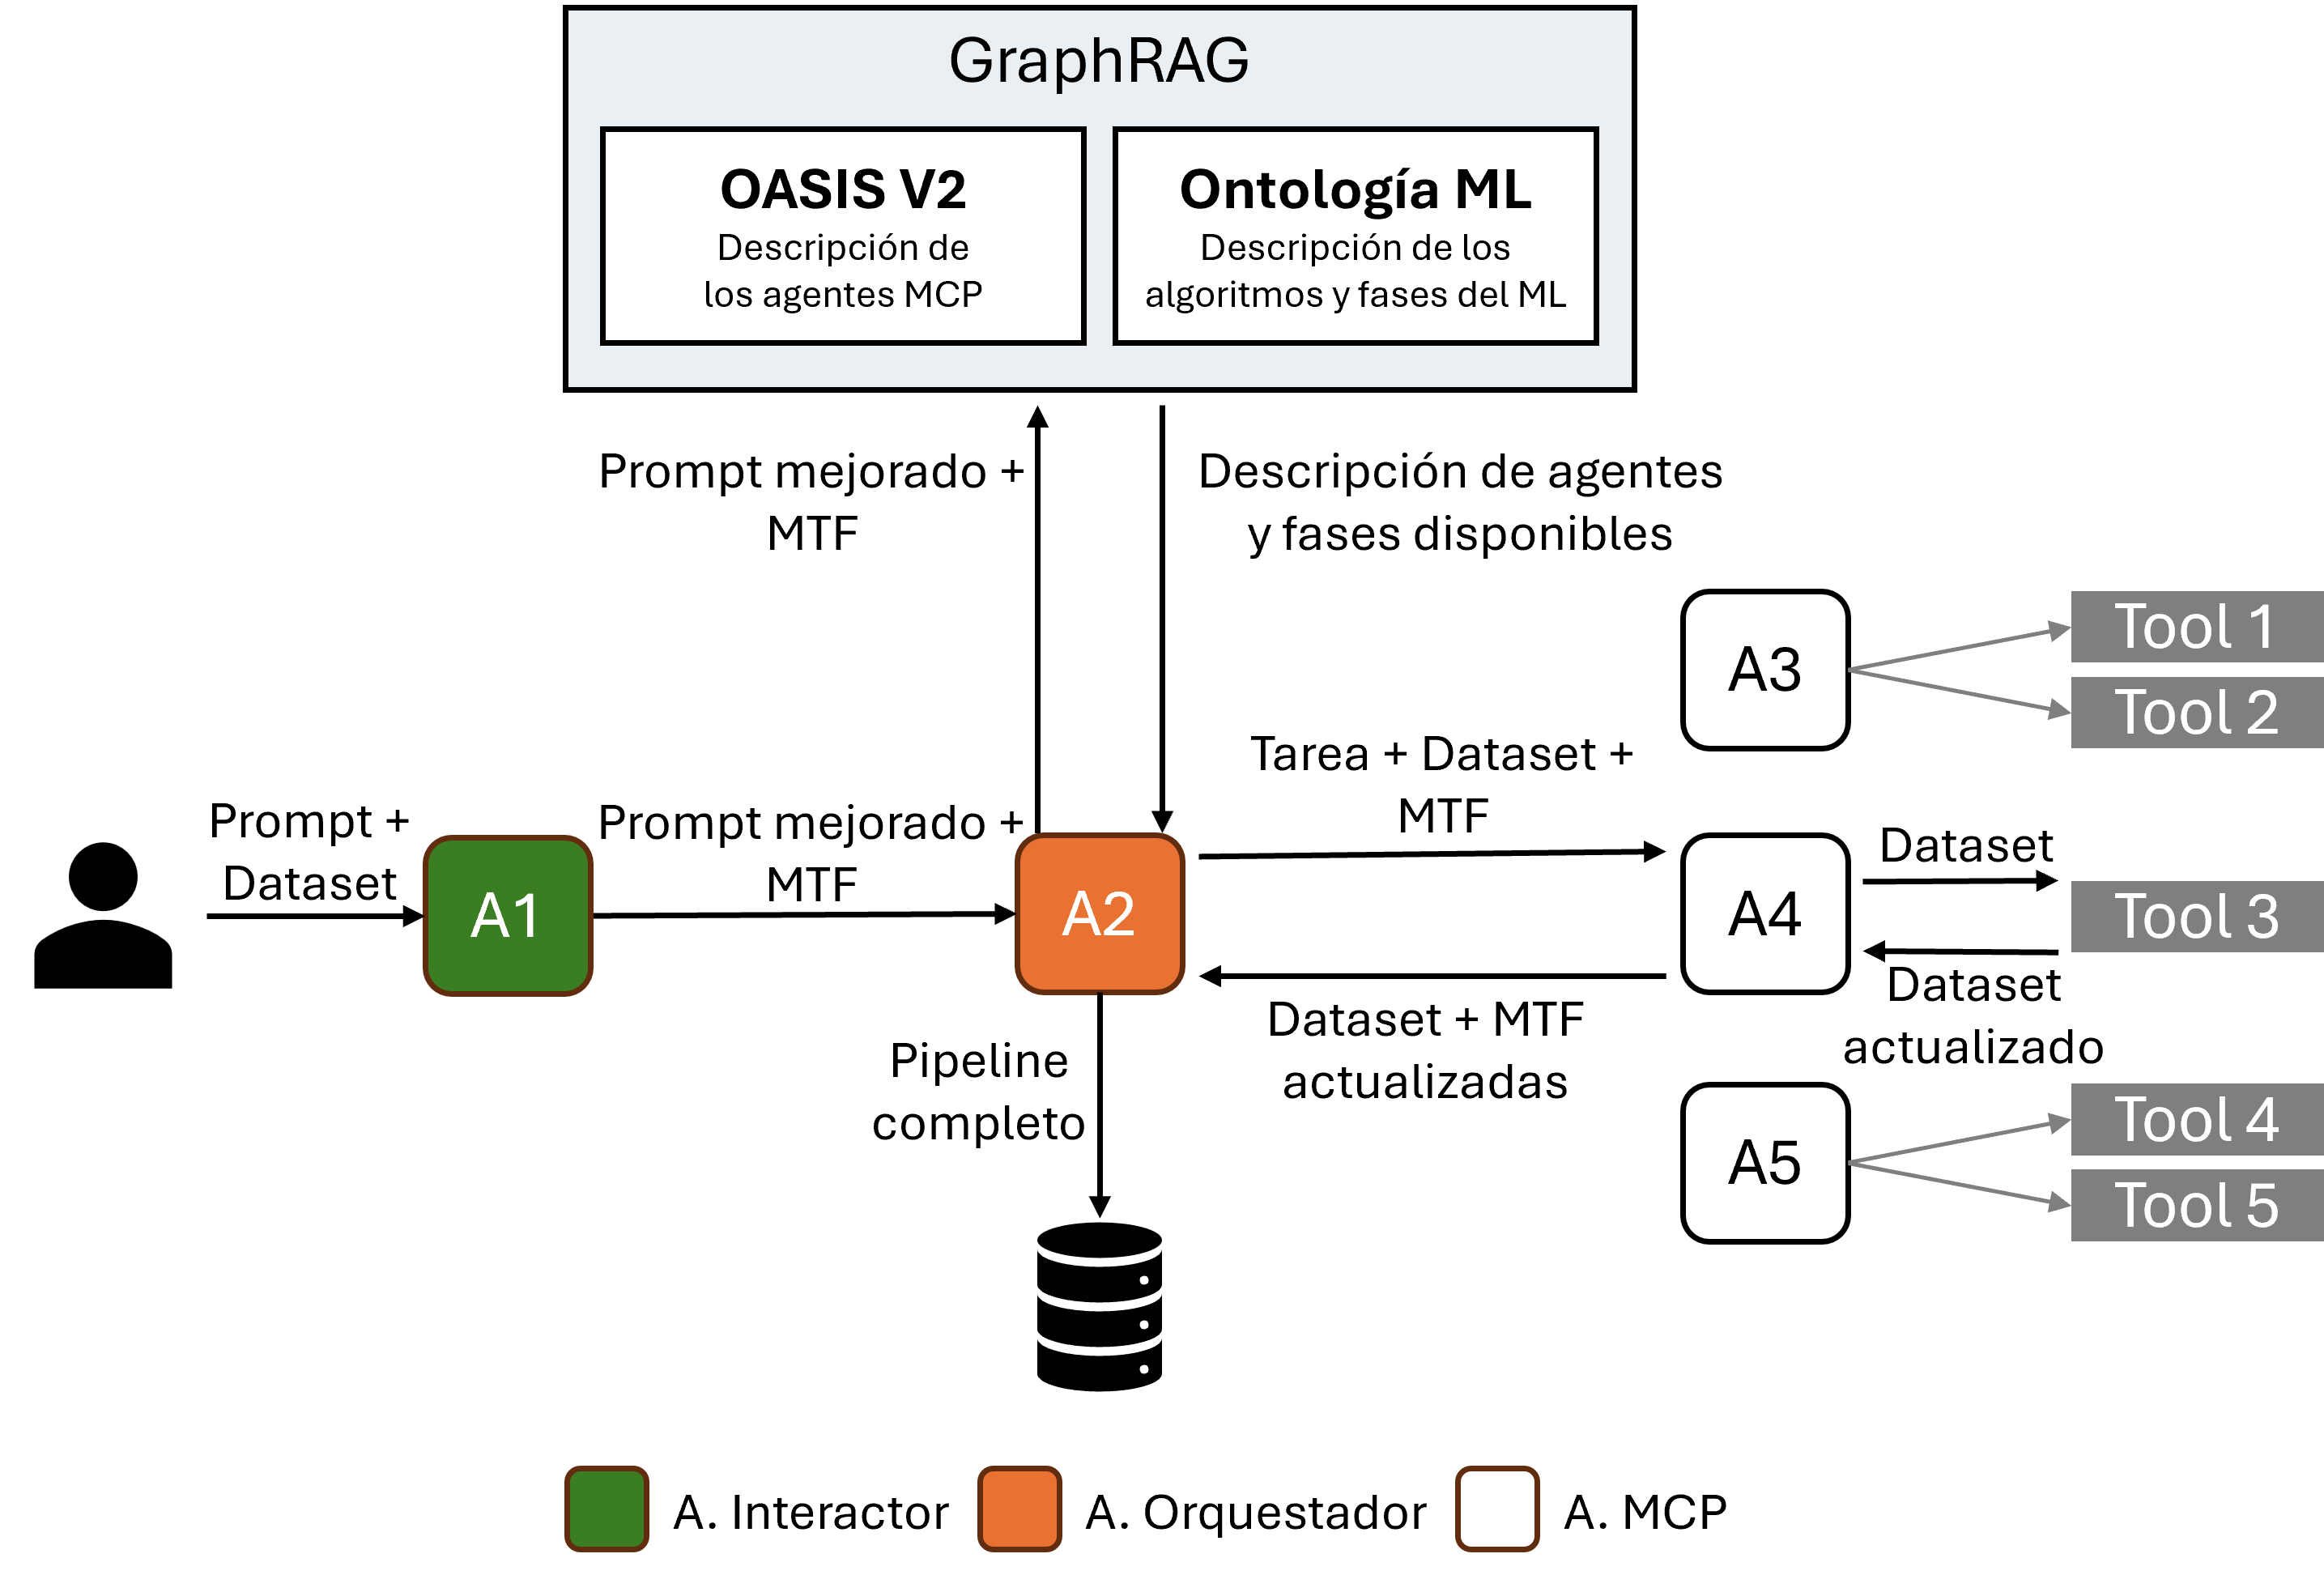
\includegraphics[width=\columnwidth]{fig/simulacion_v1.png}
\caption{Arquitectura de simulación de pipelines de ML basada en agentes MCP y GraphRAG. Los pipelines son generados mediante orquestación de agentes y exploración aleatoria, con sus ejecuciones almacenadas en una base de conocimiento para aprendizaje posterior. MTF hace referencia a las metacaracterísticas de los datasets.}
\label{fig:simulacion}
\end{figure}

El flujo de ejecución de esta parte consiste en: 

\begin{enumerate}
\item \textbf{Extracción de Metacaracterísticas y Estado (MDP):} El agente interactor (A1) recibe el conjunto de datos junto con el prompt del usuario que describe los requerimientos y el contexto del problema. A partir de esta entrada, A1 extrae las metacaracterísticas estadísticas (como dimensionalidad, correlaciones, balance de clases, entre otras) para conformar el vector numérico de estado inicial $s$ de un Proceso de Decisión de Markov (MDP)~\cite{sabbioni2023stepsize}, transfiriéndolo al orquestador (A2).

\item \textbf{Enrutamiento Ontológico Predictivo vía GraphRAG:} El Agente orquestador (A2) recibe el vector de estado y consulta semánticamente el grafo de conocimiento mediante GraphRAG. El motor de inferencia procesa las metacaracterísticas y activa restricciones axiomáticas en tiempo real, reduciendo el espacio de decisiones al bloquear agentes o transformaciones incompatibles con el dominio, como aplicar SVM a datos de tipo texto. La ontología devuelve así un conjunto restringido y seguro de fases y subtareas, garantizando la viabilidad de las etapas posteriores del pipeline.

\item \textbf{Delegación de tareas a agentes MCP:} Una vez delimitadas las opciones válidas, el orquestador (A2) delega subtareas atómicas (como imputaciones de datos, normalización, escalamiento, reducción de dimensionalidad) a agentes obreros especializados (A3 - A5). La interacción operativa y la generación de código se realiza bajo el \textit{Model Context Protocol} (MCP) utilizando herramientas externas (Tool 1-6). Este protocolo actúa como una capa de abstracción que encapsula la ejecución de código, validando su sintaxis, previniendo la corrupción del entorno computacional y devolviendo al flujo central objetos JSON estandarizados.

\item \textbf{Exploración Híbrida y Bucle de Retroalimentación:} Para evitar que los agentes se sesguen hacia secuencias convencionales, la toma de decisiones emplea una política híbrida de exploración ($\epsilon$-greedy): con probabilidad $p$ se ejecuta la acción planificada por el LLM, y con $1-p$ se selecciona una acción aleatoria pero válida según las restricciones de la ontología. Cada acción ejecutada transforma el dataset y actualiza su vector de metacaracterísticas ($s'$), permitiendo al orquestador (A2) evaluar el nuevo estado y seleccionar el siguiente paso hasta completar el pipeline. Al concluir, el desempeño del modelo (\textit{accuracy}, \textit{precision}, \textit{recall}) se asigna como una recompensa retardada ($r$) que evalúa la calidad global del pipeline.

\end{enumerate}

\subsection{Ejecución Determinista, Aprendizaje Jerárquico y Explicabilidad}

Con la base de datos poblada por millones de iteraciones de experiencia empírica, el sistema entrena un esquema de aprendizaje por refuerzo profundo jerárquico (Deep HRL). Un agente primario aprende a dictar la estructura óptima del pipeline (las herramientas a utilizar), mientras un agente secundario ajusta los hiperparámetros finos condicionados al modelo de ML y a las metacaracterísticas del dataset. Este esquema se construiría siguiendo un enfoque de recompensas multiobjetivo utilizando técnicas de vanguardia como las divergencias seccionadas estudiadas en \cite{debes2026multivariatedistributionalreinforcementlearning}, las cuales permiten acelerar el tiempo de cálculo cuando se tiene más de una recompensa asignada.

A diferencia de la simulación iterativa, la producción (figura \ref{fig:ejecucion}) es un proceso directo, eficaz y altamente explicativo:

\begin{figure}[!h]
\centering
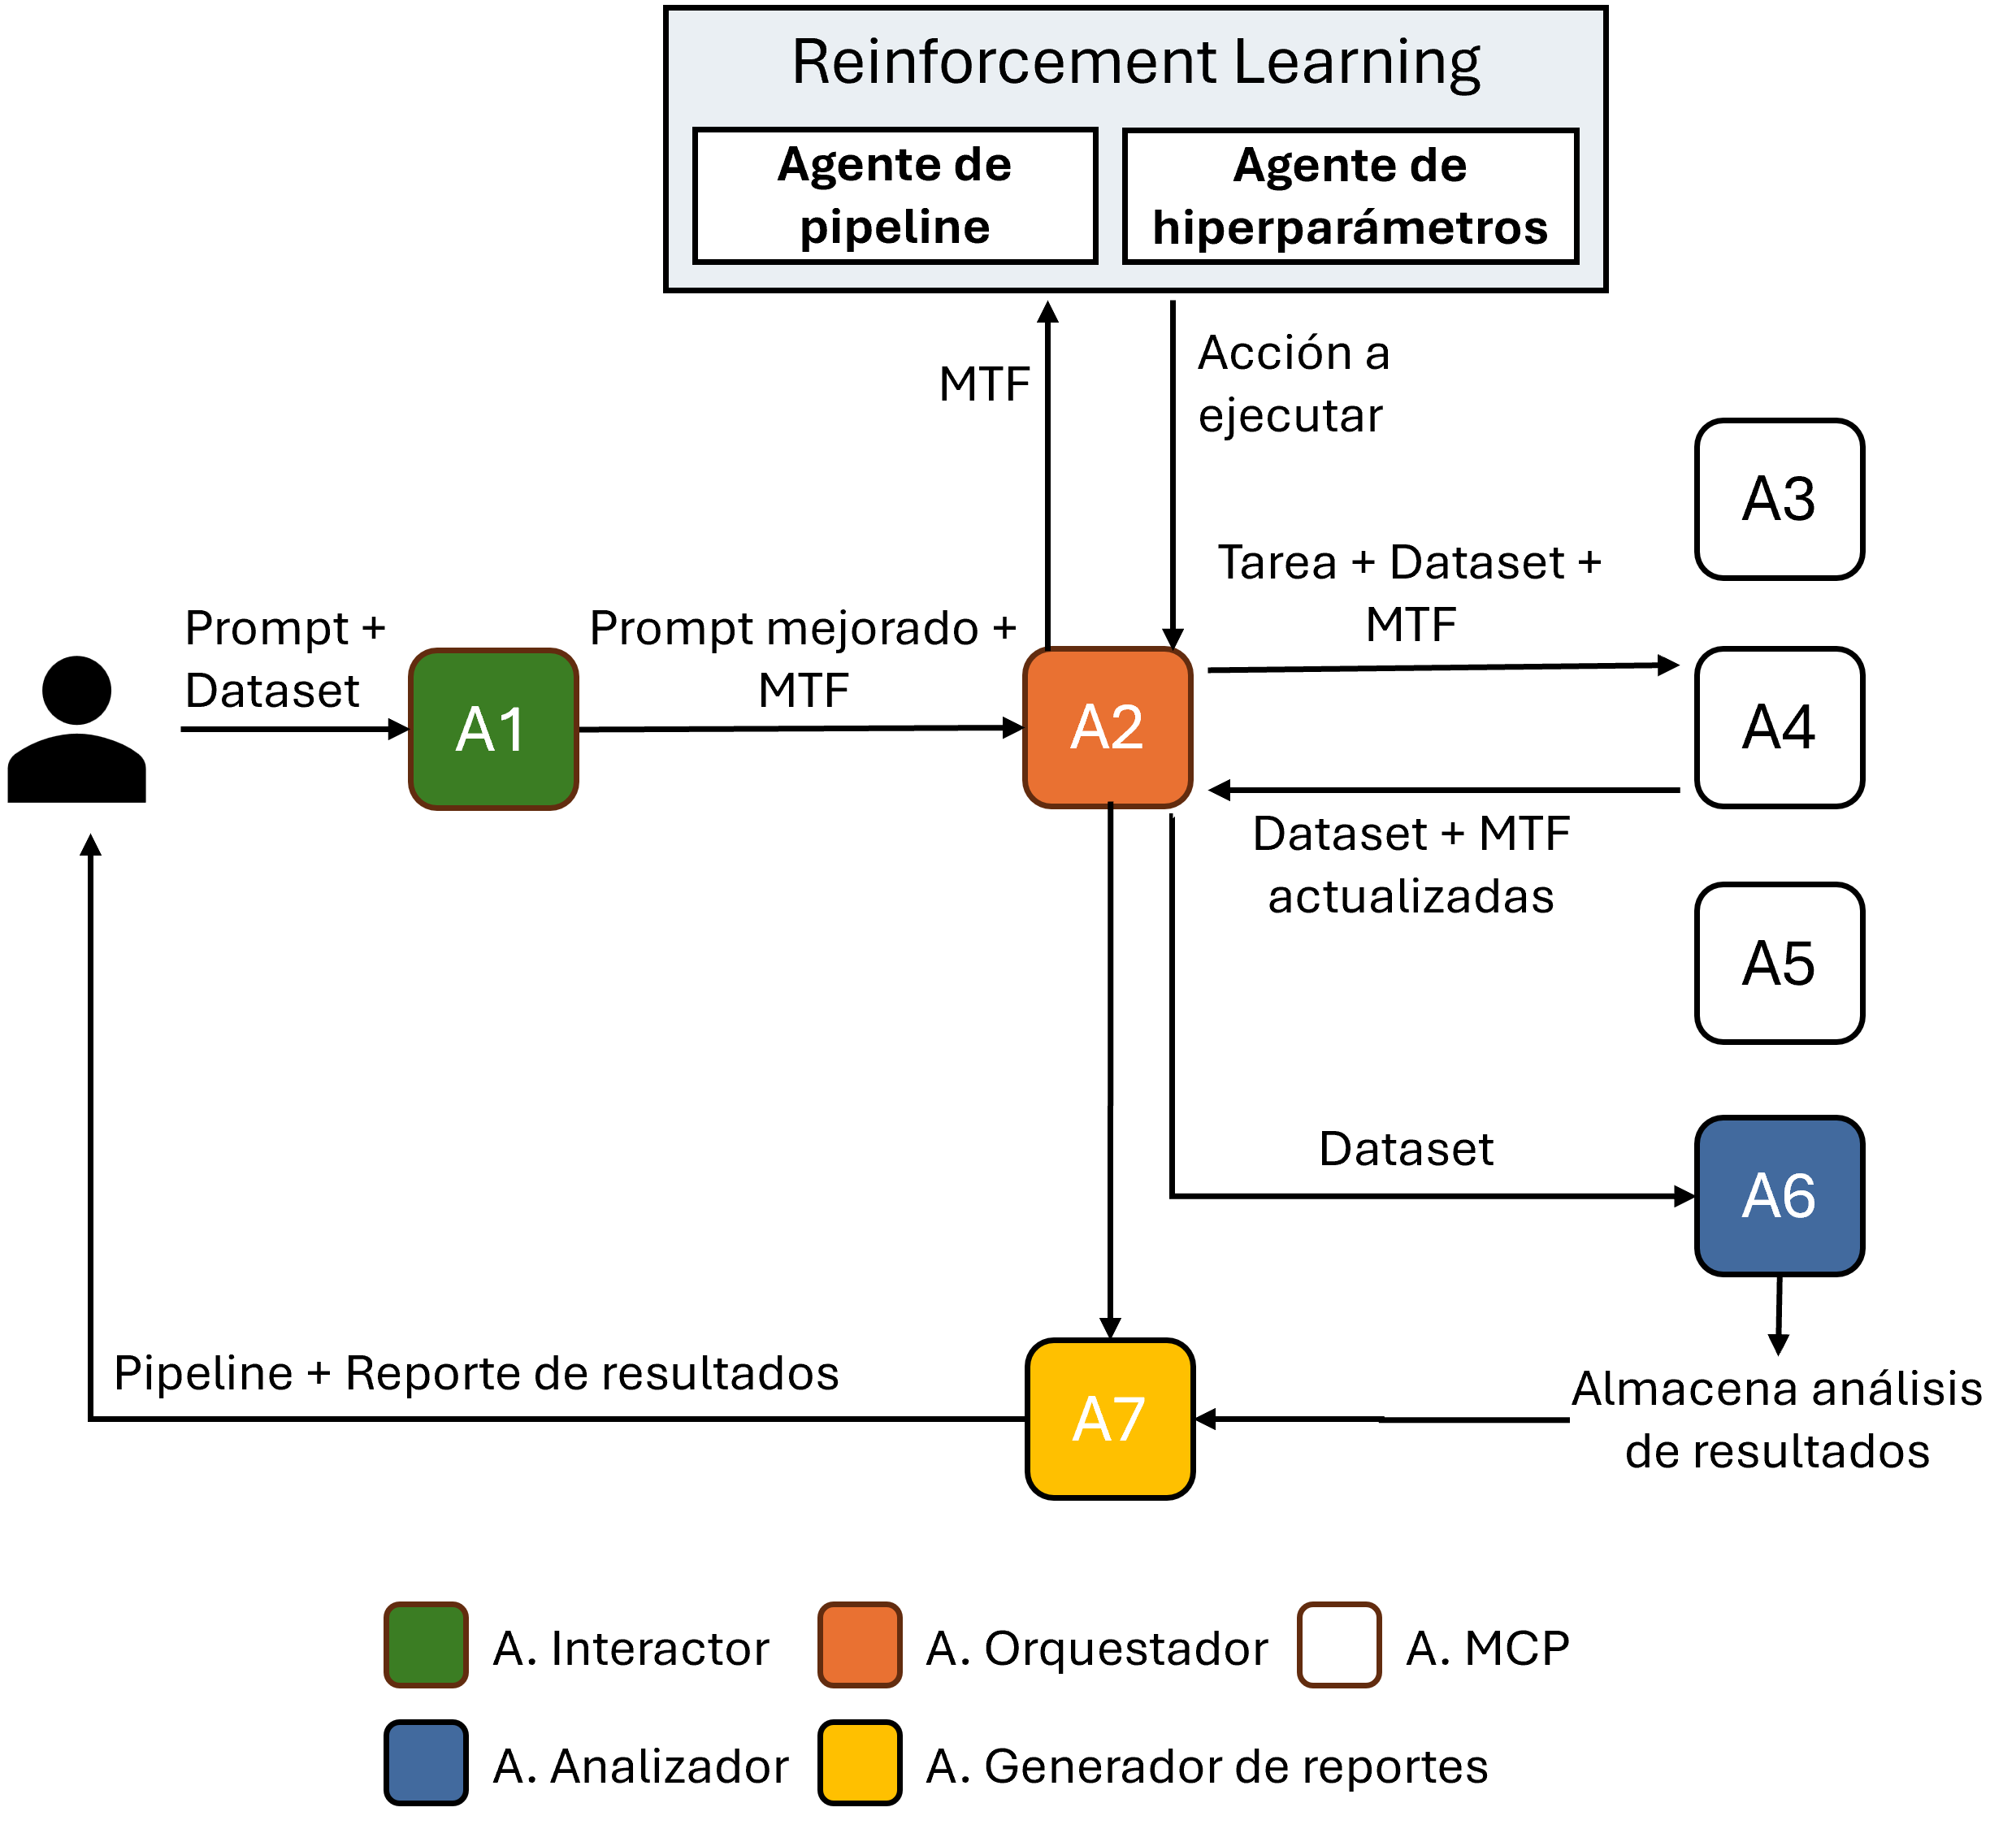
\includegraphics[width=\columnwidth]{fig/ejecucion.png}
\caption{Arquitectura de ejecución del sistema AutoML multiagéntico. El usuario proporciona un dataset y un prompt. A partir de esta información, un agente RL planifica la ejecución y optimiza los hiperparámetros, el orquestador ejecuta el pipeline y genera análisis intermedios, y un agente de reportes sintetiza el proceso, las decisiones tomadas y los principales hallazgos. MTF hace referencia a las metacaracterísticas de los datasets.}
\label{fig:ejecucion}
\end{figure}

\begin{enumerate}
\item \textbf{Ingesta y Refinamiento del Prompt:} El usuario final interactúa con la plataforma suministrando su conjunto de datos crudo junto con un prompt donde detalla el contexto operativo de los datos, las métricas de negocio prioritarias y el formato de la explicabilidad del pipeline. Un agente interactor (A1) procesa esta entrada, refinando los requerimientos del usuario, reduciendo ambigüedades y clarificando sus objetivos. Posteriormente, transforma estas especificaciones a un formato semántico estandarizado, minimizando errores de interpretación antes de iniciar la ejecución del proceso. Además de calcular las metacaracterísticas del conjunto de datos.

\item \textbf{Aplicación de la Política Óptima HRL:} El orquestador (A2) recibe el problema estructurado y, en lugar de iniciar un ciclo de búsqueda costoso, consulta de forma directa la política entrenada del agente HRL. El agente principal determina instantáneamente la configuración del pipeline idóneo basándose en las metacaracterísticas, mientras que el secundario calcula la configuración óptima de hiperparámetros. El plan de ejecución resultante se ejecuta de manera determinista a través de los agentes MCP.

\item \textbf{Puntos de Control Estratégicos de XAI:} La arquitectura rompe el secretismo de las cajas negras tradicionales mediante la activación mandatoria de un agente analizador (A6) en \textit{checkpoints} específicos del flujo del pipeline. Este agente no interviene en transformaciones triviales, sino en fases de impacto estructural como cuando el dataset se encuentra limpio y listo para realizar un análisis exploratorio de datos (EDA), cuando se ha aplicado una reducción de dimensionalidad, o cuando se ha entrenado un modelo de ML. El analizador ejecuta algoritmos estadísticos y técnicas de Inteligencia Artificial Explicable (XAI), calculando valores SHAP globales y locales para estimar la importancia de las características. Asimismo, el agente contrasta las variables más influyentes identificadas por SHAP, evaluando si las relaciones explotadas por el modelo reflejan posibles dependencias causales plausibles del dominio o meras correlaciones estadísticas del dataset.

\item \textbf{Explicación Narrativa y Auditoría Final:} Una vez consolidado el pipeline y validados los modelos, todos los artefactos, resultados gráficos generados por el agente analizador se transfieren de forma integrada al agente generador de reportes (A7). Este componente cognitivo final procesa los registros técnicos interpretando el comportamiento global del sistema para redactar de forma automatizada un informe en lenguaje natural. El reporte detalla la justificación de cada acción, la relevancia predictiva de las variables y el cumplimiento normativo, entregando al usuario una solución eficaz y auditable.

\end{enumerate}

\section{Desafíos principales}

La implementación de un sistema multiagéntico de esta complejidad plantea importantes desafíos científicos y de ingeniería. La evolución de AutoML desde enfoques basados en optimización numérica hacia sistemas dinámicos, adaptativos y explicables requiere abordar aspectos clave relacionados con la infraestructura, la coherencia del proceso de toma de decisiones y la gestión del conocimiento. Resolver estos retos será fundamental para garantizar la aplicación del sistema en entornos empresariales donde la confiabilidad y la trazabilidad sean requisitos esenciales.

El primer desafío crítico se relaciona con la elevada demanda computacional e infraestructural requerida durante la fase de simulación. La ejecución de miles de iteraciones de pipelines sobre diversos datasets, junto con el uso de LLMs para ajustar planes y orientar la exploración, puede generar costos operativos elevados. Abordar este desafío requiere el uso de infraestructuras de cómputo de altos recursos, mecanismos de optimización del uso del contexto y entornos aislados en donde las métricas de cómputo como el tiempo de ejecución no se vean alteradas por otros procesos.

Un segundo desafío se centra en la escalabilidad y actualización continua del grafo de conocimiento basado en GraphRAG y la ontología OASIS v2. A medida que el sistema incorpora nuevos agentes, y algoritmos de aprendizaje automático, la complejidad del grafo aumenta considerablemente. Esto puede afectar la eficiencia de los procesos de inferencia y consulta, por lo que será necesario desarrollar estrategias de organización del conocimiento, indexación eficiente y actualización dinámica que permitan mantener tiempos de respuesta adecuados y evitar simulaciones excesivamente largas.


El tercer desafío técnico está relacionado con la estabilidad y capacidad de generalización del esquema de HRL. La coordinación entre un agente encargado de definir la estructura general del pipeline y otro agente orientado a optimizaciones específicas, como la selección de hiperparámetros, introduce dificultades asociadas al entrenamiento y la estabilidad del aprendizaje. Para lograr que las políticas aprendidas en simulación se adapten correctamente a nuevos conjuntos de datos, será necesario diseñar mecanismos de recompensa multiobjetivo que equilibren aspectos como el desempeño predictivo, y la eficiencia computacional.


\section{Conclusiones y trabajos futuros}

En conclusión, este artículo de posición presenta un enfoque de AutoML multiagéntico orientado a superar los paradigmas actuales mediante la integración de aprendizaje por refuerzo, ontologías y agentes MCP para la generación automática de pipelines de ML trazables y auditables. Al incorporar mecanismos de explicabilidad y auditoría a lo largo de todo el proceso, la propuesta trasciende la optimización tradicional de métricas de desempeño, avanzando hacia una automatización más transparente, confiable y adaptable. De esta forma, el sistema plantea una visión de AutoML autónomo y explicable, capaz de justificar sus decisiones y comunicar el razonamiento asociado a los resultados obtenidos.

Las implicaciones prácticas de este enfoque pueden ser especialmente relevantes en entornos empresariales, donde la confiabilidad y la adaptabilidad son factores críticos. El sistema podría evolucionar no solo para generar y ejecutar pipelines de forma autónoma, sino también para operar bajo plantillas definidas por el usuario, razonar semánticamente sobre la pertinencia de determinadas técnicas según el contexto de los datos y aplicar restricciones específicas del dominio. Por ejemplo, en escenarios médicos podría identificar situaciones donde la generación de datos sintéticos implique riesgos o introduzca sesgos no deseados. Asimismo, permitiría al usuario definir qué etapas del pipeline deben ejecutarse y establecer puntos de control donde se realicen análisis estadísticos adicionales que enriquezcan el reporte final.

El objetivo futuro es iniciar la construcción del sistema descrito en este artículo y realizar experimentos que permitan evaluar su desempeño y viabilidad en escenarios reales, analizando su capacidad para generar pipelines de ML eficaces, explicables y alineados con las necesidades de los usuarios.

\bibliographystyle{IEEEtranS}
\bibliography{references}

\end{document}